\documentclass[lecture.tex]{subfiles}

\begin{document}

\exercice{}
%\video{https://youtu.be/blablabla}
\enonce{rdm-0003}{Poutre en appuie}


Soit une poutre en liaison pivot en $A$ et en appuie ponctuel en $B$. Supposant que cette poutre est chargée par une mase linéique $\rho_c = 150 \ kg/m$ et d'une masse $m=80 \ kg$ ponctuelle en $C$. Les dimensions de la poutre sont présentées dans la figure ci-dessous.

\begin{center}
  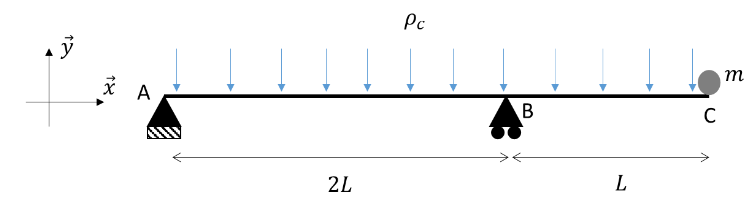
\includegraphics[scale=0.4]{exo-poutre-en-appuie.png}
\end{center}

\begin{enumerate}
  \item Faire le bilan des actions mécaniques extérieures à la poutre.
  \item Déterminer le degré d’hyperstatisme de la poutre.
  \item Trouver les inconnus de liaison de la structure (les efforts et les moments résultants de l’encastrement).
  \item Faire l’application numérique sachant que $L=1 \ m$ et $g\approx10 \ N/kg$.
\end{enumerate}

\finenonce{rdm-0003}
\finexercice


\end{document}
